%\documentclass[a4, 10 pt, conference]{ieeeconf}

\documentclass[letterpaper, 10 pt, conference]{ieeeconf}  % Comment this line out if you need a4paper

%\documentclass[a4paper, 10pt, conference]{ieeeconf}      % Use this line for a4 paper

\IEEEoverridecommandlockouts                              % This command is only needed if 
                                                          % you want to use the \thanks command

\overrideIEEEmargins                                      % Needed to meet printer requirements.

% See the \addtolength command later in the file to balance the column lengths
% on the last page of the document

% The following packages can be found on http:\\www.ctan.org
%\usepackage{graphics} % for pdf, bitmapped graphics files
%\usepackage{epsfig} % for postscript graphics files
%\usepackage{mathptmx} % assumes new font selection scheme installed
%\usepackage{times} % assumes new font selection scheme installed
%\usepackage{amsmath} % assumes amsmath package installed
%\usepackage{amssymb}  % assumes amsmath package installed


\usepackage{amssymb}
\setcounter{tocdepth}{3}
%\setlength{\parskip}{0.5ex}

\usepackage{url}
%% \urldef{\mailsa}\path|{alfred.hofmann, ursula.barth, ingrid.haas, frank.holzwarth,|
%% \urldef{\mailsb}\path|anna.kramer, leonie.kunz, christine.reiss, nicole.sator,|
%% \urldef{\mailsc}\path|erika.siebert-cole, peter.strasser, lncs}@springer.com|    
%% \newcommand{\keywords}[1]{\par\addvspace\baselineskip
%% \noindent\keywordname\enspace\ignorespaces#1}





\usepackage{cite}
 \usepackage{amsmath}
 \usepackage{amssymb}
%\usepackage{amsthm}
\usepackage{float}
\usepackage{caption}
\usepackage{algorithm}
%\usepackage{algorithmicx}
\usepackage{algpseudocode}
\usepackage{mathrsfs,amsmath}
\usepackage{graphicx}



%\setlength{\parskip}{0ex}
%\setlength{\partopsep}{0ex}
%\setlength{\parindent}{0pt} 

%\theoremstyle{plain}
\newtheorem{thm}{Theorem}[section]
\numberwithin{thm}{section} 
\newtheorem{lem}[thm]{Lemma}
\newtheorem{prop}[thm]{Proposition}
\newtheorem{cor}[thm]{Corollary}
\newtheorem{defn}[thm]{Definition}
\newtheorem{rem}[thm]{Remark}
\newtheorem{prp}[thm]{Property}
\newtheorem{prem}[thm]{Premise}
\newtheorem{egp}[thm]{Example}
\newtheorem{problem}[thm]{Problem}
%

%global macros:
\newcommand{\ra}{\rightarrow}
\newcommand{\ov}{\overline}
\newcommand{\ur}{\underline}
\newcommand{\pr}{\prime}
\newcommand{\tbf}{\textbf}
\newcommand{\omg}{\Omega}
\newcommand{\mc}{\mathcal}
\newcommand{\lt}{\left}
\newcommand{\rt}{\right}
\newcommand{\mb}{\mathbb}
\newcommand{\imp}{\implies}
\newcommand{\dimp}{\Leftrightarrow}
\newcommand{\wh}{\widehat}
\newcommand{\dg}{\mc{D}}

\newcommand{\om}{\omega}
\newcommand{\fin}{\forall i\in\{1,...,n\}}
\newcommand{\tup}[1]{\{1,...,#1\}}
\newcommand{\seq}[2]{_{#1=1}^#2}
\newcommand{\Pow}{Power}
\newcommand{\mCnn}{\mb{M}_{n\times n}(\mb{C})}
\newcommand{\mCmm}{\mb{M}_{m\times m}(\mb{C})}
\newcommand{\mCpn}{\mb{M}_{p\times n}(\mb{C})}
\newcommand{\mCnm}{\mb{M}_{n\times m}(\mb{C})}
\newcommand{\mRnn}{\mb{M}_{n\times n}(\mb{R})}
\newcommand{\mRpn}{\mb{M}_{p\times n}(\mb{R})}
\newcommand{\mRnm}{\mb{M}_{n\times m}(\mb{R})}
\newcommand{\mRno}{{{\mb{R}}}^n_{\geq 0}}
\newcommand{\mRmo}{{{\mb{R}}}^m_{\geq 0}}
\newcommand{\mRo}{\mb{R}_{\geq 0}}
\newcommand{\mRn}{{\mb{R}}^n}
\newcommand{\mRm}{{\mb{R}}^m}
\newcommand{\mCn}{\mb{C}^n}
\newcommand{\mCm}{\mb{C}^m}
\newcommand{\inv}{\mb{GL}_n(\mb{R})}
\newcommand{\id}[1]{\mb{I}_{#1\times #1}}
\newcommand{\mat}[3]{\mb{M}_{#1\times #2}(\mb{#3})}
%numbers
\newcommand{\pint}{\mb{Z}_{> 0}}
\newcommand{\nzrl}{\mb{R}_{\geq 0}}
\newcommand{\prl}{\mb{R}_{>0}}
\newcommand{\rl}{\mb{R}}

%matrix operations
\newcommand{\cjoin}[2]{\lt(\begin{array}{l}#1\\#2 \end{array}\rt)}

% local macros
\newcommand{\sw}[1]{\lt<#1,\mb{A},\Omega,\mc{I}\rt>}
\newcommand{\CZ}{\lt<V,c,s\rt>}
\newcommand{\cz}[3]{\lt<#1,#2,#3\rt>}
\newcommand{\CZO}{\lt<V,0,s\rt>}
\newcommand{\czo}[2]{\lt<#1,0,#2\rt>}
\newcommand{\sys}{\mc{S}}
\newcommand{\inp}{\Omega}
\newcommand{\mapp}{\mb{A}}
\newcommand{\init}{\mc{I}}
\newcommand{\sat}[2]{#1\vDash #2}
\newcommand{\lcons}{\lt(T,b\rt)}
\newcommand{\trj}[1]{\tbf{x}(#1)}


\title{Template complex zonotopes for stability and invariant
  verification} 

\author{Arvind Adimoolam and Thao Dang\\% <-this % stops a space
\vspace{1em}
\small{VERIMAG / CNRS, Grenoble, France} {\tt\small \{arvind.adimoolam,thao.dang\}@imag.fr}
\thanks{*This work is partially supported by the ANR MALTHY project (grant ANR-12-INSE-003)}% <-this % stops a space
%\thanks{The authors are affiliated with VERIMAG/CNRS, Grenoble, France
        %{\tt\small \{arvind.adimoolam,thao.dang\}@imag.fr}}%
}


\begin{document}
\maketitle


\begin{abstract}
Recently complex zonotopes were introduced as an extension of real
zonotopes to the complex domain, which could capture the eigenstructure
nearly periodic linear impulsive systems for stability
verification. %% They are used for stability verification of nearly
%% periodic linear impulsive systems by capturing the eigenstructure of
%% linear dynamics.
However, adding more generators to complex zonotopes distorts positive
invariance and consequently refining complex zonotopes in a verification
procedure is not easy. Therefore, in this paper we introduce a more
general set representation, called template complex zonotopes, where
the generators are fixed a-priori by a template, but the bounds on the
absolute values of their combining coefficients, called scaling
factors, are treated as variables and can be algorithmically
synthesized. %% Thus, complex zonotopes are a particular class of
%% template complex zonotopes with (fixed) unit scaling factors.
This flexibility in scaling factors leads to a more systematic and
significantly more efficient stability verification procedures in case
of template complex zonotope. Furthermore, the second contribution of
this paper is an application of template complex zonotopes to
verification of linear invariance properties of another class of
hybrid systems, namely linear switched systems with additive
disturbance. Experiments on a number of benchmark examples demonstrate
that our approach gives better or competitive results, compared to the
state-of-the-art methods and tools for these problems.
\end{abstract}

\section{Introduction}
In the design of embedded and cyber-physical systems, one of the most
important requirements is safety, which can be roughly stated as that
the system will never enter a bad state. Safety verification for such
systems are known to be computationally challenging due to the
complexity resulting from the interactions among heterogenous
components, having mixed (continuous and discrete) dynamics. In this
paper, we focus on the problem of finding invariants for hybrid
systems, which are widely recognized as appropriate for modelling
embedded and cyber-physical systems. An invariant is a property that
is satisfied in every state that the system can reach. Therefore a
common approach for proving a safety property is to find an invariant
that implies the safety property. Invariant computation has been
studied extensively in the context of verification of transition
systems and program analysis (see for
example~\cite{CousotHalbwachs78,DBLP:journals/fmsd/BensalemL99,DBLP:conf/tacas/TiwariRSS01,DBLP:conf/cav/ColonSS03,DBLP:conf/sas/Goubault13}
and the developed techniques have been extended to continuous and
hybrid
systems \cite{DBLP:conf/hybrid/SankaranarayananSM04,%% jeannet2009apron,
DBLP:conf/hybrid/Rodriguez-CarbonellT05,DBLP:conf/cdc/SassiGS14,%% DBLP:journals/tecs/AllamigeonGSGP16,
HybridFluctuat,DBLP:conf/vmcai/SogokonGJP16,DBLP:conf/aplas/DangG11}. Barrier
certificates \cite{prajna2004safety} are closely related to invariants
in the sense that they describe a boundary that the system starting
from a given initial set will never cross to enter a region containing
bad states. Another common approach to safety verification is to
compute or over-approximate the reachable set of the system, and these
reachability computation techniques have been developed for continuous
and hybrid systems.  Many such techniques are based on iterative
approximation of the reachable state on a step-by-step basis, which
can be thought of as a set-based extension of numerical integration. A
major drawback of this approach, inherent to undecidability of general
hybrid systems with non-trivial dynamics, is that such an iterative
procedure may not terminate and thus can only be used for bounded-time
safety verification (except when the over-approximation error
accumulation is not too bad that the safety can be decided). In
contrast, invariants and barrier certificates are based
on conditions that are satisfied at all times. Although solving these
conditions often involves fixed point computation, by exploiting the
structure of the dynamics (such as eigenstructures of linear systems),
one can derive meaningful conditions which can significantly reduce
the number of iterations until convergence.



For discrete time affine hybrid systems, the eigenvectors of the
products of linear matrices related to the affine dynamics of
different subsystems can possibly capture some of the stable
directions for the overall hybrid dynamics.  As such, for invariant
computation, template complex zonotopes have the advantage that they
can include the possibly complex eigenvectors among the generators,
while usual (real) zonotopes can not.  In an earlier
work~\cite{tcz2017}, numerically efficiently solvable conditions for
computing a template complex zonotopic invariant subject to linear
safety constraints were obtained for a limited class of hybrid
systems, i.e., having uncontrolled switching.  However, a formidable
hurdle in extending the approach for more general affine hybrid
systems, where switching is controlled by linear constraints, is that
we have to handle the intersection of template complex zonotopes with
the linear constraints.  In this regard, template complex zonotopes
share the drawback of usual zonotopes that these classes of sets are
not closed under intersection with linear constraints.

In this paper, we circumvent this problem as follows.  We observe that
it is possible to compute or reasonably overapproximate the
intersection of a template complex zonotope with a class of linear
constraints, called subparallelotpic, by appropriately choosing the
template of the complex zonotope.  We use a slightly more general set
representation, called augmented complex zonotope, with which the
intersection operation can be succinctly presented.  %% Geometrically
%% speaking, augmented complex zonotopes and template complex zonotopes
%% describe the same classes of sets in terms of their real valued
%% projections.  However, it is easier and more succinct, using the
%% representation of an augmented complex zonotope instead of a template
%% complex zonotope, to represent the resultant intersection with linear
%% constraints. 
Then, we derive a numerically efficiently solvable
sufficient condition for computing an augmented complex zonotopic
invaraint satisfying linear safety constraints, for a discrete time
affine hybrid system with subparallelotopic switching constraints and
bounded additive disturbance input.  The sufficient condition is
expressed as a set of second order conic constraints.  We also note
that the class of sub-parallelotopic constraints that we consider are
quite general and can be used in the specification of many examples of 
affine hybrid systems.  To corroborate our approach by presenting the
experimental results for three benchmark examples from literature.
%% We implemented our approach on three benchmark examples from
%% literature and compared the results with that of the SpaceEx tool
%% on the same discrete time models, and also the reported benchmark
%% results from literature.  In some experiments, we could verify
%% finite safety bounds when SpaceEx could not even find an
%% invariant. In other experiments, we could verify competitive safety
%% bounds.  Also, our computation time is quite reasonable in all the
%% experiments, depending on the size of the specification.



\emph{Related work.} For hybrid systems verification, convex polyhedra~\cite{CousotHalbwachs78,jeannet2009apron}, and their special classes such as
%% zones~\cite{DBLP:conf/pado/Mine01},
octagons~\cite{DBLP:journals/lisp/Mine06} and
zonotopes~\cite{DBLP:conf/hybrid/Girard05,DBLP:conf/eucc/MaigaCRT14}
and tropical polyhedra~\cite{DBLP:conf/sas/AllamigeonGG08} are the
most commonly used set representations. During reachability analysis,
which requires operations under which a set representation is not
closed (such as the union or join operations for convex polyhedra and
additionally intersection for zonotopes), the complexity of generated
sets increases rapidly in order to guarantee a desired error
bound. One way to control this complexity increase is to fix the face
normal vectors or generators, which leads to template convex
polyhedra \cite{Sankaranarayanan+Dang+Ivancic-08-Symbolic,DBLP:conf/aplas/DangG11}. Although
our template complex zonotopes proposed in~\cite{tcz2017} do not
belong to the class of convex polyhedra, they follow the same spirit
of controlling the complexity using templates. Set representations
defined by non-linear constraints include
ellipsoids~\cite{Kurzhanski2000201}, polynomial
inequalities\cite{DBLP:conf/sas/BagnaraRZ05} and
equalities~\cite{Rodriguez-Carbonell:2007}, quadratic templates and
piecewise quadratic templates~\cite{%% DBLP:conf/esop/AdjeGG10,
DBLP:conf/hybrid/RouxJGF12,DBLP:conf/fm/RouxG14,DBLP:conf/hybrid/Adje17},
which are used for computing non-linear invariants. A major problem of
template based approaches finding good templates.  In this regard,
using template complex zonotopes and the augmented version introduced
in this paper, we can exploit eigen-structures of linear dynamics
which reflect the contraction or expansion of a set by the dynamics,
and define good templates for efficient convergence to an invariant
(see Proposition 4.3 of~\cite{adimoolamACC2016}).

The extension to complex zonotope~\cite{adimoolamACC2016} is
very similar in spirit to quadratic
zonotopes~\cite{DBLP:conf/aplas/AdjeGW15} and more generally
polynomial zonotopes~\cite{DBLP:conf/hybrid/Althoff13}. Nevertheless,
while a polynomial zonotope is a set-valued polynomial function
of \emph{intervals}, a complex zonotope is a set-valued function of
unit \emph{circles} in the complex plane.  Our idea in this paper of coupling
additional linear constraints with complex zonotopes is inspired by the work
on constrained zonotopes proposed
in~\cite{DBLP:conf/cav/GhorbalGP09,scott2016constrained} for computing
intersection with linear constraints.  But
while~\cite{DBLP:conf/cav/GhorbalGP09,scott2016constrained} compute
the intersection or its overapproximation, algorithmically, we instead
derive a simple algebraic expression to overapproximate the
intersection.  This algebraic expression is latter used to obtain
second order conic (convex) constraints, for invariant computation in
a single step of convex optimization.

\emph{Organization.}  The rest of the paper is organized as follows.  Firstly, we explain
some of the mathematical notation used in this paper.  Then in
Section~\ref{sec:system}, we describe the model of a discrete-time
affine hybrid system, controlled by sub-parallelotopic switching
conditions and having a bounded additive disturbance input. In
Section~\ref{sec:acz}, we present the set representation of augmented
complex zonotopes and discuss some important operations and relations,
in particular intersection with sub-parallelotopic constraints,
projection in any direction, linear transformation, Minkowski sum and
inclusion checking.  In Section~\ref{sec:invcomp}, we derive a set of
second order conic constraints to compute an augmented complex
zonotopic invariant, satisfying linear safety constraints and
containing an initial set.  Furthermore, we explain how to choose the
template.  In Section~\ref{sec:exp}, we report some experimental
results.  The conclusion and future work are given in
Section~\ref{sec:conclusion}.
%% We annex proofs of some lemmas presented in the paper in an
%% Appendix.

\emph{Notation.} Some notations for which we
consider explanation may be required is described below.  We denote
$\comprealset = \realset\bigcup\lt\{-\infty,\infty\rt\}$.  If $S$ is a
set of complex numbers, then $\real(S)$ and $\img(S)$ represent the
real and imaginary projections of $S$, respectively.  If $z$ is a
complex number, then $|z|$ denotes the absolute value of $z$.  On the
other hand, if $X$ is a complex matrix (or vector), then $\lt|X\rt|$
denotes the matrix (or vector) containing the absolute values of the
elements of $X$.  The diagonal square matrix containing the entries of
a complex vector $z$ along the diagonal is denoted by $\dg(z)$.  The
conjugate transpose of a matrix $V\in\mat{m}{n}{\complexset}$ is
denoted $\conjtranspose{V} = \lt(\real(V)-\iu\img(V)\rt)^T.$ If
$V\conjtranspose{V}$ is invertible, then
$\pinv{V}= \conjtranspose{V}\lt(V\conjtranspose{V}\rt)^{-1}$, which is
the pseudo-inverse of $V$.  Given two vectors $l,u\in\realset^k$ and
any relation $\bowtie$ between numbers in $\comprealset$, we say
$l\bowtie u$ if $l_i\bowtie u_i,~\forall i\in\tup{k}$.  The meet of
the two vectors $l$ and $u$ is denoted $l\bigwedge u$, defined as
$\lt(l\bigwedge u\rt)_i=\min\lt(l_i,u_i\rt)~\forall i\in\tup{k}$.  The
join is denoted $l\bigvee u$, defined as $\lt(l\bigvee
u\rt)_i=\max\lt(l_i,u_i\rt)~\forall i\in\tup{k}$.





\section{Template complex zonotopes}~\label{sec:tcz}
\paragraph{\bf Definition.}
A template complex zonotope is a set representation in which each point
is described as a linear combination of a set of complex-valued vectors,
called as a \textit{template}, such that the complex combining coefficients are
bounded in absolute values by a set of positive bounds called
\textit{scaling factors}.
%
\begin{defn}[Template complex zonotope]
  For $n,m\in\pint$, let $V\in\mCnm$ be a template, $c\in\mCn$
  be a center point and $s\in\mRmo$ be scaling factors.  Then we
  define a template complex zonotope as 
  \[\cz{V}{c}{s}=\lt\{V\zeta+c:\zeta\in\mCm~\wedge~\forall
  i\in\{1,\ldots,m\},|\zeta_i|\leq s_i\rt\}.\]
\end{defn}
%
Complex zonotopes, which were introduced in~\cite{arvind2016lis}, are
a special case of template complex zonotopes where $s_i = 1$ for all
$i\in\{1,...,m\}$.  The real projection of a template complex zonotope
can represent, in addition to polytopic zonotopes, non-polyheral
convex sets.  Therefore, they are also more expressive than usual
(real-valued) zonotopes.  To illustrate, Figure~\ref{fig:cz}
represents the non-polyhedral real projection of the template complex
zonotope $\CZO$ where $V=\lt(\begin{array}{lll}(1+2i) & 1 &
  (2+i)\\(1-2i) & 1 & (2-i)\end{array}\rt)$ and $s=[1~1~1]^T$.
%
\begin{figure}
\center
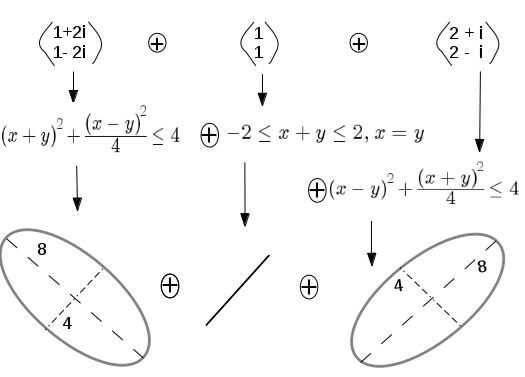
\includegraphics[scale=0.7]{fig/complex-zonotope.png}
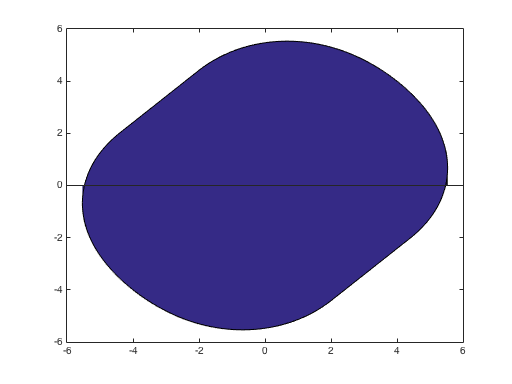
\includegraphics[scale=0.5]{fig/CZhull.png}
\caption{Real projection of a template complex zonotope}
\label{fig:cz}
\end{figure}
%




In the rest of the paper, unless otherwise stated, we assume that $V$
is an $n\times m$ complex matrix, $s$ is an $m\times 1$ column vector
and $c$ is a $n\times 1$ column vector for $m,n\in\pint$.

\paragraph*{\bf Operations on template complex zonotopes}
Concerning linear transformation and the Minkowski sum, computations
on template complex zonotopes are similar to those on usual (real-valued) zonotopes
as stated in the following results, which can be proved by the same
techniques as that of a usual zonotope. %~\cite{todo}.
%
\begin{lem}[Linear transformation and Minkowski sum]~\label{lem:lt}
  Let $A\in\mCnn$, $V\in\mCnm$, $G\in\mat{n}{r}{C}$, $c,d\in\mCn$, $s\in\mRmo$,
  $h\in\mb{R}^r_{\geq 0}$ for some $n,m,r\in\pint$.
  
\begin{enumerate}%\begin{equation}\label{eqn:lin} 
\item \emph{Linear transformation}: $A\CZ=\cz{AV}{Ac}{s}$.
\item \emph{Minkowski sum}: $\CZ\oplus\cz{G}{d}{h}=\cz{\lt[V~~G\rt]}{(c+d)}{\lt(\begin{array}{l}s\\h\end{array}\rt)}$.
%\end{equation}
\end{enumerate}
\end{lem}
%% \begin{proof}
%% $A\CZ=\{A(V\zeta +c):
%% |\zeta_i|\leq s_i~\forall i\in\tup{m}\}=\cz{AV}{Ac}{s}$.
%% \end{proof}
%
%% The Minkowski sum of two template complex zonotopes is another
%% template complex zonotope computed as follows.
%% %
%% \begin{lem}[Minkowski sum]\label{prop:op}
%%   Let $V\in\mCnm$, $G\in\mat{n}{r}{C}$, $c,d\in\mCn$, $s\in\mRmo$,
%%   $h\in\mb{R}^r_{\geq 0}$ for some $n,m,r\in\pint$.  Then
%% \begin{equation}\label{eqn:msum}
%% \CZ\oplus\cz{G}{d}{h}=\cz{\lt[V~~G\rt]}{(c+d)}{\lt(\begin{array}{l}s\\h\end{array}\rt)}
%% \end{equation}
%% \end{lem}
%% \begin{proof}
%% $\CZ\oplus\cz{G}{d}{h}\\=\{V\zeta+G\zeta^\pr+c+d:|\zeta_i|\leq s_i\forall
%% i\in\tup{m}~\wedge~|\zeta^\pr_j|\leq h_j\forall j\in\tup{r}\}\\
%% =\lt\{[V~~G]\cjoin{\zeta}{\zeta^\pr}+(c+d):|\zeta_i|\leq s_i\forall
%% i\in\tup{m}~\wedge~|\zeta^\pr_j|\leq h_j\forall
%% j\in\tup{r}\rt\}\\=\cz{\lt[V~~G\rt]}{(c+d)}{\cjoin{s}{h}}$.
%% \end{proof}


Checking inclusion is a fundamental problem in reachability
computation. For stability verification, we are interested in
efficiently checking the inclusion between two template complex
zonotopes centered at the origin.  Although this problem is non-convex
in general, we derive an easily verifiable convex condition which is
sufficient (but not necessary), as follows.  The inclusion checking
method we propose in the following can be extended to zonotopes
centered anywhere.


Let us consider that we want to check the inclusion of a template
complex zonotope $\czo{V^a}{s^a}$ inside a template complex zonotope
$\czo{V^b}{s^b}$, where $V^a\in\mat{n}{r}{C}$, $V^b\in\mCnm$,
$s^a\in\mb{R}^{r}_{\geq 0}$ and $s^b\in\mb{R}^m_{\geq 0}$ for some
$n,m,r\in\pint$.  We relate any point in $V^a$ to a point in $V^b$ as
follows.  Consider $X\in\mat{r}{m}{C}$ as a matrix solving
$V^a\dg(s^a)=V^bX$, which we call a \emph{transfer matrix} from
$\czo{V^a}{s^a}$ to $\czo{V^b}{s^b}$.  Recall that $\dg(s^a)$ is the
diagonal square matrix containing entries of $s^a$ along its
diagonal. Let any point $z$ in $\czo{V^a}{s}$ be written as
$z=V^a\zeta$ where $\zeta$ is a combining coefficient whose absolute
values are bounded by $s^a$.  By normalizing with the scaling factors,
we can write $\zeta=\dg(s)\epsilon$ for some
$\epsilon:\|\epsilon\|_{\infty}\leq 1$.  So, we get
$z=V^a\dg(s)\epsilon$.  Then using the relation for the transfer
matrix, we rewrite $z=V^bX\epsilon$.  If the absolute value of every
component of $X\epsilon$ is less than the corresponding value of
$s^b$, then $X\epsilon$ can be treated as a combining coefficient of
$\czo{V^b}{s^b}$ for the point $z$ and then $z$ also belongs to
$\czo{V^b}{s^b}$.  This is true if $\sum_{j=1}^m|X_{ij}|\leq
s^b_i~\forall i\in\tup{m}$.  This gives us a sufficient condition,
stated in the following theorem for inclusion of $\czo{V^a}{s^a}$ in
$\czo{V^b}{s^b}$.

%
\begin{thm}[Inclusion]\label{thm:inc}
   Let $V^a\in\mat{n}{r}{C}$, $V^b\in\mCnm$, $s^a\in\mb{R}^{r}_{\geq
     0}$ and $s^b\in\mb{R}^m_{\geq 0}$ for some $n,m,r\in\pint$.  Then
   $\czo{V^a}{s^a}\subseteq \czo{V^b}{s^b}$ if all the following
   statements are true.   
\begin{align}
\begin{split}
& \exists X\in\mat{m}{r}{C}:~\\
& V^bX=V^a\dg(s^a)~~\text{and}~~\forall i\in\tup{m}~~\lt(\sum_{j=1}^r|X_{ij}|\rt)\leq s_i^b.
\end{split}
\end{align}
\end{thm}


For fixed $V_a$ and $V_b$, the constraints in Theorem~\ref{thm:inc}
are second order conic constraints in the variables $s^a$, $s^b$ and
$X$.  Many convex optimization solvers can solve such constraints can
efficiently upto a high numerical precision.



 
\section{Nearly periodic linear impulsive system}\label{sec:lis}
A nearly periodic linear impulsive system is a hybrid system
whose state evolves continuously by a linear differential equation
for some bounded time period, after which there is an instantaneous
linear impulse.  Formally, a linear impulsive system is specified by
a tuple $\mc{L}=\left<A_c,A_r,\Delta\right>$ where $A_c$ and $A_r$ are
$n\times n$ real matrices called the linear field matrix and impulse
matrix, respectively.  The positive integer $n$ is the dimension of
the state space and $\Delta=[t_{min},t_{max}]$ is an interval of
non-negative reals, called the sampling period interval.  The
dynamics of the nearly periodic linear impulsive system is described
as follows.  A function
$\tbf{x}:\mathbb{R}_{\geq 0}\ra \mathbb{R}^n$ is called a trajectory
of the system if there exists a sequence of sampling times
$(t_i)_{i=1}^\infty$ satisfying all the following:
%
	\begin{equation}\label{eqn:system} \begin{split}
&(t_{i+1}-t_i)\in\Delta~~\forall i\in\pint~~~~(\text{uncertainty in sampling period})\\
&\dot{\tbf{x}}(t)=A_c\tbf{x}(t)~~\forall
            t\in\nzrl:~t\neq t_i ~\forall i\in\pint~~(\text{continuous
              })\\
&\tbf{x}(t_i^+)=A_r\tbf{x}(t_i^-)~~\forall
            i\in\pint~~~~(\text{linear impulse})           
\end{split} \end{equation}
%
%% 	Here $\tbf{x}(t)\in\mathbb{R}^n$ is the state of the system at a time instant
%% $t$.  We denote the set of all possible trajectories of the system by $\Gamma$.
%% \vspace{0.2em}

We say that the linear impulsive system is globally exponentially
stable (GES) if all the trajectories of the system beginning at any
point in the state space eventually reach arbitrarily close to the
origin at an exponential rate, as %% Formally, GES is defined as
follows.
%
\begin{defn}[Global exponential stability]
  The system~(\ref{eqn:system}) is
  globally exponentially stable (GES) if there exist positive scalars
  $c>0$ and $\lambda\in[0,1)$ such that for all $t\in\mRo$,
  $\trj{t}\leq c\lambda^t\|\trj{0}\|$.
\end{defn}
We state the stability verification problem as follows.
%
\begin{problem}[Stability verification problem]
Given $A_c$, $A_r$, $t_{min}$, find the largest upper bound $t_{max}$ on the sampling time to guarantee exponential stability.
\end{problem}
%

\paragraph*{Related work on stability verification of nearly periodic linear impulsive systems} 

%A general approach to verifying exponential
%stability of nearly-periodic linear impulsive systems is to find
%decreasing Lyapunov functions
%~\cite{2013-briat-convex,Mikheev1988,Teel1998,2010-liu-stability,Mazenc2013,2010-fridman-refined}. If
%the Lyapunov functions are quadratic, they can be reduced to Linear
%Matrix Inequality (LMI) conditions~\cite{HetelDaafouz2006}.  Another
%approach is to find contractive
%sets~\cite{2014-fiacchini-set,Lazar2013,AlKhatib2015}, which is the
%inspiration to our work.  


A common approach to this problem is extending Lyapunov techniques, which results in Lyapunov Krakovskii functionals 
\cite{Mikheev1988,Teel1998} (using the framework of time-delay systems), and discrete-time Lyapunov functions \cite{2012-seuret-novel}. Stability with respect to time-varying input delay can also be handled by input/output approach 
\cite{DBLP:conf/amcc/KaoW14}. Stability verification problem for time-varying impulsive systems can also be formulated in a hybrid systems framework \cite{nevsic2004framework,Goebel2009,BauLoo_NECSYS12a}, for which various Lyapunov-based 
methods including discontinuous time-independent \cite{2008-naghshtabrizi-exponential} 
or time-dependent Lyapunov functions \cite{2010-fridman-refined} were developed. Another approach involves using convex embedding \cite{HetelDaafouz2006,Fujioka2009,2013hetel}. In this approach, stability conditions can be checked using parametric Linear Matrix Inequalities (LMIs) \cite{HetelDaafouz2006}, 
or as set contractiveness (such as, polytopic set contractiveness) \cite{2014-fiacchini-set,2013-briat-convex,AlKhatib2015}. Inspired by these results on 
set contractiveness conditions~\cite{arvind2016lis} provides a stability condition, expressed in terms of complex zonotopes, which is more conservative but can be efficiently verified. The novelty of this work is in the extension of complex zonotopes to template complex zonotopes which allows a systematic way to synthesize contractive zonotopic sets to verify stability. 

%Computationally speaking, our approach is close in spirit to abstract interpretation
%and hybrid systems analysis. Indeed the way we find contractive sets using such zonotopes is similar 
%to the way invariant sets are computed using some zonotopic
%\cite{Girard05reachabilityof,Althoff2011,DBLP:conf/sas/GoubaultPV12} and
%template-polyhedral abstract domains \cite{S riram2008,jeannet2009apron}.

%\cite{DBLP:conf/amcc/KaoW14,Omran2013}


%% To show exponential stability, we use reachability analysis as
%% follows.  Beginning at a state $x$ and by continuous evolution for a
%% time period $t$, the system reaches the state $e^{A_ct}x$, which we
%% obtain by integrating the continuous dynamics of the system.  On the
%% other hand, after a linear impulse at a state $x$, the system reaches
%% the state $A_rx$.  Overall, 

The state reached after a linear impulse followed by a continuous
evolution for time $t$ is $e^{A_ct}A_rx$.  So, let us denote
$H_t=e^{A_ct}A_r$ for any any positive real $t$, which we call as the
reachability operator if $t$ lies in the sampling period interval
$\Delta$.  Given a set $\Psi\subset\mathbb{R}^n$, the set of all
reachable points of $\Psi$, when acted upon by an impulse followed by
continuous evolution for sampling time period $t\in\Delta$ until
before the next impulse, is $\bigcup_{t\in\Delta}H_t\Psi$.  It was
shown previously in~\cite{2014-fiacchini-set,AlKhatib2015} that a
necessary and sufficient condition for exponential stability is the
existence of a convex, compact and closed set containing the origin in
its interior, called a $C$-set, that contracts between subsequent
impulses.  In other words, we can establish exponential stability by
finding a $C$-set $\Psi$ such that $H_t\Psi\subseteq\lambda\Psi$ for
some $\lambda\in[0,1)$ and for all $t\in\Delta$.  In this paper, we
  want to find contractive $C$-sets represented as template complex
  zonotopes.  We define \emph{contraction} of a
template complex due to a linear operator as follows, which when less
than one, implies that the zonotope is contractive.
%
\begin{defn}
For a template complex zonotope $\CZO$, the amount of contraction by a
square matrix $J\in\mat{n}{n}{R}$, denoted by $\chi(V,s,J)$
is \[\chi(V,s,J)=\min\lt\{\lambda\in\mRo:J\czo{V}{s}\subseteq
\lambda\czo{V}{s}\rt\}.\]
\end{defn}
%
Our motivation of for considering
template complex zonotopes can be
inferred from the following proposition.  
%
\begin{prop}~\label{prop:eig-cont}
  Let $V$ contain only the eigenvectors of $H_t$ as its column vectors
  and $\mu$ be the vector of eigenvalues corresponding the columns of
  $V$.  Then $H_t\CZO=\czo{V}{\dg(|\mu|)s}$.
\end{prop}
%
For a fixed sampling time period, i.e., when $t_{min}=t_{max}=t$, we
can infer from the above proposition that the contraction of the
template complex zonotope formed by the eigenvector template is
bounded by the largest absolute value of the eigenvalues.  
Therefore, when the sampling period is fixed, we can find contractive
template complex zonotopes for exponentially stable systems by
choosing the template as the collection of eigenvectors.  However, we
are interested in the case where the sampling time period varies in
the interval $\Delta$, i.e. there are uncountably many reachability
operators parametrized over the time interval $\Delta$. Motivated by
the above analysis, when the sampling period is uncertain, we choose
the template as the collection of eigenvectors of a few reachability
operators and try to synthesize suitable scaling factors for which the
template complex zonotope contracts with respect to the chosen finite
set of reachability operators.  However, later we also verify that the
synthesized template complex zonotope actually contracts with respect
to all the (uncountably many) reachability operators.  First we
describe the procedure to synthesize the template complex zonotope.

 \emph{Synthesizing a candidate template complex
  zonotope.} This step of systematically synthesizing a suitable
template complex zonotope that is likely to be contractive constitutes
the main improvement over the procedure proposed
in~\cite{arvind2016lis}. Our criterion for synthesizing the template
complex zonotope is that it has to be contractive with respect to a
few reachability operators (called reference operators), which is a
necessary condition for contraction with respect to the overall system
dynamics.  Since the eigenstructure of the reachability operators are
related to the stability of the system, we include the eigenvectors of
a few reachability operators in the template.  For a fixed number
$k\in\pint$ of reference operators, they can be chosen incrementally
as follows.  Define $k$-sampled time points as
$\Lambda_k=\lt\{t_{min}+i\frac{(t_{max}-t_{min})}{k}:i\in\{0,\ldots,k-1\}\rt\}.$
Then we define the set of $k$-sampled reachability operators as
$\Gamma_k=\lt\{H_{t}:t\in\Lambda_k\rt\}$.  Let us denote the template
of collection of eigenvectors of all operators in $\Gamma_k$ as $E_k$.
For this template, we synthesize suitable scaling factors based on the
following theorem. The derivation of this theorem uses the inclusion
checking condition from Theorem~\ref{thm:inc}.
%
\begin{thm}
If $E_k$ have rank $n$.  For a
vector of scaling factors $s\in\mb{R}^{m}_{\geq 0}$, the template
complex zonotope $\mc{Z}=\czo{E_k}{s}$ would represent a $C$-set and also $H_t\mc{Z}\subseteq
\lambda\mc{Z}$ for $\lambda\in(0,1)$ if
following are all satisfied.
%
\begin{equation}\label{eqn:syn}
\begin{split}
& s\in\mb{R}^n_{\geq 1}~~\text{(sufficient condition for representing $C$-set)}\\
& \exists X_t\in\mat{m}{m}{C}~~\forall t\in\Lambda_k~~\text{s.t.}\\
& E_kX_t=H_tE_k\dg(s)~~~~(\text{transfer matrix condition
    })\\%~(\text{a finite set of time points})\\
& \sum_{j=1}^m\lt|\lt(X_t\rt)_{ij}\rt|\leq \lambda s_i~~\forall i\in\tup{m}~~\text{(bounding contraction)}\\
\end{split}
\end{equation}
\end{thm}

Therefore, we can synthesize a template complex zonotope that is
contractive with respect to a finite chosen number $k>0$ of reference
operators by solving for the scaling factors satisfying the
second-order conic constraints in~(\ref{eqn:syn}).

\emph{Verifying contraction.}  To verify that this synthesized
template complex zonotope actually contracts with respect to all the
reachability operators $H_t$, where $t$ is parametrized over the whole
sampling time interval $\Delta$, we divide the sampling interval into
small enough sub-intervals and verify contraction in each interval.
To bound the amount of contraction in small intervals, we use some
useful properties of contraction, which were earlier derived
in~\cite{arvind2016lis}.

Let $H_{t+\rho}$ be an operator where $\rho$ lies in the interval
$(0,\epsilon)$.  For an order of taylor expansion $r\in\pint$ and some
$\delta\in[0,\epsilon]$, define 
\[P^t_r(\rho)=\sum_{i=0}^r\frac{A_c^i\rho^i}{i!}H_t~~\text{and}~~
E^t_r(\delta)=\frac{A_c^{r+1}\delta^{r+1}}{(r+1)!}H_t.\]  Then based
on Taylor expansion, we get that \[H_{t+\rho} = P_r^t(\rho) +
E_r^t(\delta).\]
%
Furthermore, a bound on contraction as sum of contractions depending on $\epsilon$ is derived 
in~\cite{arvind2016lis} as
%
\begin{equation}\label{eqn:expbound}
\begin{split}
&~~~~~~~~~~~\chi\lt(V,s,H_{t+\rho}\rt)\leq
\lt(\max_{i=0}^r\chi\lt(V,s,P^t_r(\epsilon)\rt)\rt)+ \frac{\epsilon^{r+1}}{(r+1)!}\chi\lt(V,s,A_c^{r+1}H_t\rt)
\end{split}
\end{equation}
%
The right hand side of~(\ref{eqn:expbound}) can be bounded if we know
a bound on the contraction under a linear operation, which is
derived as follows.
%
\begin{lem}\label{lem:contLin}
Let $J\in\mRnn$.  Define 
\[\beta(V,s,J)=\min\{\|X\|_\infty:X\in\mat{m}{m}{C}~\wedge~
V\dg(s)X=JV\dg(s)\}\] Then we have $\chi(V,s,J)\leq \beta(V,s,J)$.
%
\end{lem}
\begin{proof}
If $JV\dg(s)=V\dg(s)X$, we want to prove that $J\czo{V}{s}=\czo{JV}{s}\subseteq \|X\|_\infty\CZO$.  We deduce
$\czo{JV}{s}=\{ JV\zeta \;:\; \forall
  i\in\tup{m}|\zeta_i|\leq s_i \} = \{JV\dg(s)\zeta^\pr:\|\zeta^\pr\|_{\infty} \leq 1\} = \{V\dg(s)X\zeta^\pr:\|\zeta^\pr\|_\infty\leq 1\}\subseteq
  \|X\|_\infty\{V\dg(s)\zeta^\pr:\|\zeta^\pr\|_{\infty}\leq
  1\} = \|X\|_\infty\{V\zeta \;:\; \forall i\in\tup{m}  |\zeta_i|\leq s_i \} = \|X\|_{\infty}\CZO$.
\end{proof}
%
Then the contraction for sampling time interval $(t,t+\delta)$ can be
bounded %% using Equations~(\ref{eqn:expbound}) and Lemma~(\ref{lem:contLin})
as follows.
%
\begin{thm}\label{thm:expbound}
  Let $\rho\in (t,t+\epsilon)$ and for $r\in\mb{Z}_{>0}$, $
  P^t_r(\rho)=\sum_{i=0}^r\frac{A_c^i\rho^i}{i!}H_t$.  Define
  $\eta_r(V,s,t,\epsilon)=
  \lt(\max_{i=0}^r\beta\lt(V,s,P^t_r(\epsilon)\rt)\rt)+
  \frac{\epsilon^{r+1}}{(r+1)!}\beta\lt(V,s,A_c^{r+1}H_t\rt)$, where
  the bound $\beta(.)$ is defined in Lemma~\ref{lem:contLin}.  Then
  $\chi\lt(V,s,H_{t+\rho}\rt)\leq \eta_r(V,s,t,\epsilon) $
\end{thm}
%
\emph{Verification algorithm.} We begin with $k=3$ reference operators
that correspond to the two end points of the sampling interval and the
middle point.  The algorithm first finds suitable scaling factors $s$
that gives a template complex zonotope which contracts with respect to
these reference operators.  Next, it checks whether the contraction of
the template complex zonotope $\czo{E_k}{s}$ with respect to all the
reachability operators is less than one. For checking contraction, we
use the algorithm earlier proposed in ~\cite{arvind2016lis}.  If
successful, then exponential stability of the system is verified.
Otherwise, $k$ is increased, the algorithm synthesizes the template
complex zonotope for the increased $k$ and then checks contraction. If
unsuccessful after a maximum value of $k$, the algorithm stops and the
result is inconclusive.  This is described in
Algorithm~\ref{alg:1step}. This algorithm has been implemented and
we defer experimental results to Section~\ref{sec:exp}.
%
 \begin{algorithm}
\caption{Exponential stability verification of system~(\ref{eqn:system})}
\label{alg:1step}
\begin{algorithmic}[1]
\State Initialize $k=3$.
\State Choose $M\in\pint$ as the largest value of $k$ and $tol$ as
discretization parameter.
\While{$k \leq M$}
\State Initialize $t=t_{min}$, $h=tol$, $r$ as order of Taylor
expansion (typically $\leq 2$).
\While{$h\geq \; tol$ and $t<t_{max}$}
\If{$\eta_r(E_k,s,t,h)<1$}
\State $t\gets t+h; h\gets h+tol$
\Else
\State $h\gets h-tol$
\EndIf
\EndWhile
\If{$t\geq t_{max}$}
\State {\bf|BreakLoop|}
\Else
\State $k\gets k+1$.  
\EndIf
\EndWhile
\If {$k \leq M$}
\State \emph{System is exponentially stable}
\Else
\State \emph{Inconclusive}
\EndIf
\end{algorithmic}
\end{algorithm}




In a discrete time affine hybrid system, the state of the system is
specified by a discrete valued variable, called location, and a
continuous variable whose valuation is in the real Euclidean space of
a finite dimenstion.  The state of the system in each location has to
stay within a polyhedral set, called the staying condition.  The state
of the system can change by two kinds of transitions, {\it continuous
  transition} and {\it discrete transiton}.  In a continuous
transition, the discrete state of the system remains constant while
the continuous state changes by an affine transformation.  The affine
transformation has possible additive disturbance input, which is
bounded.  The parameters of the affine transformation of a continuous
transition depend on the location in which the transition takes place.
In a discrete transition, there is a change in the discrete variable
accompanied by an affine transformation of the continuous variable.
The transition is has precondition specified by a linear constraint,
called a guard, while the post-condition is the staying condition in
the location reached after transition.  A set of edges specifies
the possible discrete transitions, vis a vis, the locations between
which a discrete transition takes place, the parameters of the affine
transformation and the guard.   

{\it Sub-parallelotopic guards and staying conditions}: In this paper,
we consider hybrid systems where the guards and staying conditions can
be specified by a sub-parallelotope with a common template.  We note
that the class of sub-parallelotopic constraints are quite general and
can be used in the specification of many practical affine hybrid
systems.  

{\bf Model.}  We specify the discrete time affine hybrid system
by a tuple 
 %
\[
\system = \lt(\locations,\qtemp,\stay,\linmap,\inputset,\edgeset,\Psi\rt).
\]
%
The finite set of locations is $\locations$.  The sub-parallelotopic
template for specifying the guards and staying conditions is
$\qtemp\in\mat{k}{n}{\reals}$.  The staying set in a location
$\loc\in\locations$ is a sub-parallelotope
$\ptope{\qtemp}{\lsys{\stay_\loc}}{\usys{\stay_\loc}}$, whose pair of
lower and upper interval bounds is
$\stay_\loc=\lt(\lsys{\stay_\loc},\usys{\stay_\loc}\rt)$ .  The
parameters affine transformation in a location $\loc\in\locations$
consist of a linear transformation, specified by a matrix
$\linmap_\loc\in\mat{n}{n}{\reals}$, and a bounded additive
disturbance input set $\inputset_\loc\subset\reals^n$.  The set of
edges is $E$.  An edge $\edge\in\edgeset$ is specified by a tuple
%
\[
\edge=\lt(\edge_1,\edge_2,\usys{\edge},\lsys{\edge},\linmap_\edge,\inputset_\edge\rt).
\]
%
The before and after locations of a discrete transition along an edge
$\edge$ are $\edge_1,\edge_2$.  The guard on the transition along the
edge $\edge$ is the sub-parallelotope
$\ptope{\qtemp}{\lsys{\edge}}{\usys{\edge}}$, whose pair of
lower and upper interval bounds is
$\lt({\lsys{\edge}},{\usys{\edge}}\rt)$.
The parameters of the affine transformation for the discrete
transition along the edge $\edge$ consists of a linear map specified
by the matrix $\linmap_\edge\in\mat{n}{n}{\reals}$ and a bounded
additive disturbance input set $\inputset_\edge\subset\reals^n$.  The
set of initial states of the system is $\Psi\subseteq\locations\times\reals^n$.

{\bf Dynamics.}  A state of the hybrid system is a pair $(x,\loc)$,
where $x\in\reals^n$, called the {\it continuous state}, and
$\loc\in\locations$, called the {\it discrete state}.  A {\it
  trajectory} specifies the evolution of the state of the system as a
function of discrete time instants.  A trajectory is a function
$\maphtrj:\integers_{\geq 0}\ra\reals^n\times\locations$, such that
$\forall t\in\integers_{\geq 0}$, one of the following conditions is
true.
%
\begin{enumerate}
\item todo
\item todo
\end{enumerate}
%































{\color{red} TODO.}  

\section{Experiments} \label{sec:exp}
\emph{Computation platform.} For convex optimization, we use CVX
version 2.1 with Matlab R2015a.  The reported experimental results were
obtained on 64 bit GNOME (3.4.2) with Intel Core i5-3470 CPU, 3.20GHz
processor, having 3.8 GiB memory and disk space 242.1 GB.





\subsection{Nearly periodic linear impulsive systems}\label{sec:lis-ex}
%Experiments for linear impulsive systems

We evaluated the implementation of our algorithm on a number of
benchmark examples taken from~\cite{arvind2016lis} and compared it
with the state-of-the-art methods and tools and our algorithm produced
either better or competitive results.  We describe two of the examples
for linear impulsive systems below.

\emph{Example 1.} We consider a networked control system with
uncertain but bounded transmission period.  A networked control system
is composed of a plant and a controller that interact with each other
by transmission of feedback input from controller to the plant.  If
the system dynamics is linear with linear feedback, then for uncertain
but bounded transmission period, we can equivalently represent it
as a linear impulsive system where $A_c=\lt(\begin{array}{ccc} A_p & 0 & B_p\\ 0 & 0 &
  0\\ 0 & 0 & 0
\end{array}\rt),~A_r=\lt(\begin{array}{ccc}
\mb{I} & 0 & 0\\
B_oC_p & A_o & 0\\
D_oC_p & C_o & 0
\end{array}\rt)$ for some parameter matrices $A_p$, $B_p$, $B_o$,
$C_p$, $A_o$, $C_o$, and $D_o$.  The sampling interval $\Delta$ of the
linear impulsive system specifies bounds on the transmission interval.
%
Our example of a networked control system is taken from Bj\"{o}rn et
al.~\cite{wittenmark2002computer}.  The system is originally described
by discrete time transfer functions, which has an equivalent state
space representation with parameter matrices
$A_p=\lt(\begin{array}{cc}-1 & 0\\ 1 & 0\end{array}\rt)$,
  $B_p=\lt(\begin{array}{c}1\\ 0\end{array}\rt)$,
    $C_p=\lt(\begin{array}{cc}0 & 1\end{array}\rt)$, $A_o=0.4286$,
      $B_o=-0.8163$, $C_o=-1$ and $D_o=-3.4286$.  Given the lower
      bound on the transmission period as $t_{min}=0.8$, we want to
      find as high a value of $t_{max}$ as possible for which the
      system is GES.

\emph{Example 2.} We consider the following linear impulsive system
from Hetel et. al.~\cite{2013hetel}, that describes an LMI based
approach to verify stability. The specification is given by
$A_c=\left(\begin{array}{ccc} 0 & -3 & 1\\ 1.4 & -2.6 & 0.6\\ 8.4 &
  -18.6 & 4.6
\end{array}\rt)
$ and $A_r=\lt(\begin{array}{ccc} 1 & 0 & 0\\ 0 & 1 & 0\\ 0 & 0 & 0
\end{array}\rt).$

While implementing the algorithm for stability verification, we choose
first order Taylor expansion, $tol=0.05$ for Example 1 and $tol=0.006$
for Example 2.  We required $k=3$ as the number of reachability
operators used for synthesis of a suitable template complex zonotope
for stability verification in both examples.  Then we verified
stability in a sampling interval $[0.08, 0.5]$ for Example 1 and
$[0.1,0495]$ for Example 2.  Our approach is compared with the
state-of-the-art NCS toolbox~\cite{BauLoo_NECSYS12a} and also other
approaches as listed in Table~\ref{tab:com1} and Table~\ref{tab:com2}.
For the first example, our method outperforms other approaches, while
it is competitive with other approaches on the second example.
Moreover, Table~\ref{tab:tcz-cz} shows that the template complex
zonotopic approach is computationally more efficient than complex
zonotopes~\cite{arvind2016lis}.

\begin{table}
\begin{minipage}{0.49\textwidth}
\caption{Example 1}
\begin{tabular}{|l|c|r|}
  \hline
  Reference & $t_{min}$ & $t_{max}$ \\
\hline
  %& &\\
Value recommended in~\cite{wittenmark2002computer} & 0.08 & 0.22\\
  \hline
  %& &\\
  NCS toolbox~\cite{BauLoo_NECSYS12a} & 0.08 & 0.4 \\
  \hline
  %& &\\
Complex zonotope~\cite{arvind2016lis} & 0.08 & 0.5 \\
\hline
  %& &\\
  Template complex zonotope & 0.08 & 0.53 \\
  \hline
\end{tabular}
\label{tab:com1}
\end{minipage}
\begin{minipage}{0.49\textwidth}
\caption{Example 2}
\label{tab:com2}
\begin{tabular}{|l|c|r|}
\hline
    Reference & $t_{min}$ & $t_{max}$ \\
  \hline
  %& &\\
  Lyapunov, parametric LMI~\cite{2013hetel} & 0.1 & 0.3 \\
  \hline
  %& &\\
  Polytopic set contractiveness~\cite{2014-fiacchini-set} & 0.1 & 0.475 \\
  \hline
  %& &\\
Khatib et al.~\cite{AlKhatib2015} & 0.1 & 0.514\\
\hline
  %& &\\
Complex zonotope~\cite{arvind2016lis} & 0.1 & 0.49 \\
\hline
 % & &\\
  Template complex zonotope & 0.1 & 0.496 \\
  \hline
\end{tabular}
%\label{tab:com2}
\end{minipage}
\vspace{1em}
\caption{Template complex zonotopes (TCZ) vs
    Complex zonotopes (CZ)~\cite{arvind2016lis}}
\center
 \begin{tabular}{|l|c|r|}
  \hline
  $~$ & CZ & TCZ $~~~~~~~~$\\
  \hline
  Finding suitable zonotope & Requires guessing & Systematically synthesized\\
\hline
  No. of impulses for contraction & 2 (both examples) & 1 (both examples)\\
  \hline
    Computation time (Example 1) & 27.41 s & 4.6 s \\
\hline
Computation time (Example 2) & 74.04 s & 8.5 s\\
\hline
\end{tabular}
\label{tab:tcz-cz}
\end{table}














%\vspace{-em}
\section{Conclusion}
\vspace{0em}
We extended complex zonotopes to template complex zonotopes in order to
improve the efficiency of the computation of contractive sets and
positive invariants.  Template complex zonotopes retain a useful feature of complex zonotopes, which is the scope to incorporate the
eigenvectors of linear dynamics among the generators because the
eigenstructure is related to existence of positive
invariants.  In addition, compared to complex zonotopes, the advantage
template complex zonotopes have is the ability to regulate the
contribution of each generator to the set by using the scaling factors.
This resulted in significantly improved verification of stability of
nearly periodic impulsive systems, and also extending its application
to switched systems for verification of linear invariance properties.
The advantage of this new set representation is attested
by the experimental results that are better or competitive, compared
to the state-of-the-art methods and tools on benchmark examples. This
work also contributes a method for exploiting the eigenstructure of
linear dynamics to algorithmically determine template directions,
required by most verification approaches using template sub-polyhedral
sets. A number of directions for future research can be
identified. First, we intend to extend these techniques to analysis to
switched systems under constrained switching laws. Also
computationally speaking, our approach is close in spirit to abstract
interpretation. Indeed the operations used to find positive invariants and contractive sets
can be extended to invariant computation for more general hybrid
systems with state-dependent discrete transitions.
%to the way invariant sets are computed using some zonotopic

%and hybrid systems analysis. Indeed the way we find contractive sets using such zonotopes is similar 
%to the way invariant sets are computed using some zonotopic
%\cite{Girard05reachabilityof,Althoff2011,DBLP:conf/sas/GoubaultPV12} and
%template-polyhedral abstract domains \cite{S riram2008,jeannet2009apron}.


%\bibliographystyle{plain}
%\bibliography{ref,domain,mprt}



\begin{thebibliography}{10}

\bibitem{arvind2016lis}
A. Adimoolam and T. Dang.
\newblock Using complex zonotopes for stability verification.
\newblock In {\em American Control Conference}.
  sites.google.com/site/cztopepubs/, 2016.

\bibitem{AdjeGaubertGoubaultESOP2010}
A.~Adje, S.~Gaubert, and E.~Goubault.
\newblock Coupling policy iteration with semi-definite relaxation to compute
  accurate numerical invariants in static analysis.
\newblock In {\em ESOP}, volume 6012, pp 23--42, 2010.

\bibitem{DBLP:conf/aplas/AdjeGW15}
A. Adj{\'{e}}, P.{-}L .Garoche, and A. Werey.
\newblock Quadratic zonotopes - an extension of zonotopes to quadratic
  arithmetics.
\newblock In {\em APLAS 2015}, pp 127--145, 2015.

\bibitem{DBLP:conf/sas/AllamigeonGG08}
X. Allamigeon, S. Gaubert, and E. Goubault.
\newblock Inferring min and max invariants using max-plus polyhedra.
\newblock In {\em SAS}, LNCS 5079, pp 189--204.
  {Springer}, 2008.

\bibitem{allamigeon2015scalable}
X. Allamigeon, S. Gaubert, E. Goubault, S. Putot, and
  N. Stott.
\newblock A scalable algebraic method to infer quadratic invariants of switched
  systems.
\newblock In {\em Embedded
  Software}, pp 75--84. IEEE Press, 2015.

\bibitem{althoff2013}
M. Althoff.
\newblock Reachability analysis of nonlinear systems using conservative
  polynomialization and non-convex sets.
\newblock In {\em HSCC 2013}, pp 173--182. ACM, 2013.

\bibitem{bagrodzafSAS05}
R.~Bagnara, E.~Rodr{\'\i}guez-Carbonell, and E.~Zaffanella.
\newblock Generation of basic semi-algebraic invariants using convex polyhedra.
\newblock In {\em SAS 2005},
LNCS 3672, pp 19--34, Springer-Verlag, 2005.

\bibitem{BauLoo_NECSYS12a}
N.W. Bauer, S.J.L.M. van Loon, M.C.F. Donkers, N~van~de Wouw, and W.P.M.H.
  Heemels.
\newblock Networked control systems toolbox: Robust stability analysis made
  easy.
\newblock In {\em IFAC Workshop on Distributed Estimation and Control in
  Networked Systems (NECSYS)}, pp 55--60, 2012.

\bibitem{blanchini2015switching}
F. Blanchini and S. Miani.
\newblock Switching and switched systems.
\newblock In {\em Set-Theoretic Methods in Control}, pp 405--466. Springer,
  2015.

\bibitem{2013-briat-convex}
C. Briat.
\newblock Convex conditions for robust stability analysis and stabilization of
  linear aperiodic impulsive and sampled-data systems under dwell-time
  constraints.
\newblock {\em Automatica}, 49(11):3449--3457, 2013.

\bibitem{Cai2008}
C. Cai, R.~Goebel, and A.R. Teel.
\newblock Smooth lyapunov functions for hybrid systems part ii:
  (pre)asymptotically stable compact sets.
\newblock {\em IEEE Trans. on Automatic Control}, 53(3):734--748, 2008.

\bibitem{CousotCousot76-1}
P. Cousot and R. Cousot.
\newblock Static determination of dynamic properties of programs.
\newblock In {\em 2nd Int. Symp. Prog.}, pp 106--130. Dunod, 1976.

\bibitem{DBLP:conf/popl/CousotH78}
P. Cousot and N. Halbwachs.
\newblock Automatic discovery of linear restraints among variables of a
  program.
\newblock In {\em POPL}, pp 84--96, 1978.

\bibitem{DBLP:conf/aplas/DangG11}
T. Dang and T.M. Gawlitza.
\newblock Template-based unbounded time verification of affine hybrid automata.
\newblock In {\em APLAS 2011}, LNCS 7078, pp 34--49. Springer, 2011.

\bibitem{Feron2010}
E.~Feron.
\newblock From control systems to control software: Integrating
  lyapunov-theoretic proofs within code.
\newblock {\em IEEE Control Systems Magazine}, (1):50--71, December 2010.

\bibitem{2014-fiacchini-set}
M. Fiacchini and I.-C. Morarescu.
\newblock Set theory conditions for stability of linear impulsive systems.
\newblock In {\em CDC 2014}, IEEE, 2014.

\bibitem{2010-fridman-refined}
E. Fridman.
\newblock A refined input delay approach to sampled-data control.
\newblock {\em Automatica}, 46(2):421--427, 2010.

\bibitem{Fujioka2009}
H. Fujioka.
\newblock A discrete-time approach to stability analysis of systems with
  aperiodic sample-and-hold devices.
\newblock {\em IEEE Trans. on Aut. Control}, 54(10):2440--2445,
  2009.

\bibitem{HSCC05}
A. Girard.
\newblock Reachability of uncertain linear systems using zonotopes.
\newblock In {\em HSCC}, pp 291--305, 2005.

\bibitem{Goebel2009}
R.~Goebel, R.G. Sanfelice, and A.~Teel.
\newblock Hybrid dynamical systems.
\newblock {\em Control Systems, IEEE}, 29(2):28--93, 2009.

\bibitem{HetelDaafouz2006}
L.~Hetel, J.~Daafouz, and C.~Iung.
\newblock Stabilization of arbitrary switched linear systems with unknown
  time-varying delays.
\newblock {\em IEEE Trans. on Automatic Control}, 51(10):1668--1674,
  2006.

\bibitem{2013hetel}
L. Hetel, J. Daafouz, S. Tarbouriech, and C. Prieur.
\newblock Stabilization of linear impulsive systems through a nearly-periodic
  reset.
\newblock {\em Nonlinear Analysis: Hybrid Systems}, 7(1):4--15, 2013.

\bibitem{Hu2003}
L.~Hu, J.~Lam, Y.~Cao, and H.~Shao.
\newblock A  {LMI} approach to robust h2 sampled- data control for linear
  uncertain systems.
\newblock {\em IEEE Trans. Syst. Man Cybern.}, 33(1):149--155, 2003.

\bibitem{DBLP:conf/amcc/KaoW14}
C.{-}Y. Kao and D.{-}R. Wu.
\newblock On robust stability of aperiodic sampled-data systems - an integral
  quadratic constraint approach.
\newblock In {\em ACC 2014}, pp 4871--4876, 2014.

\bibitem{AlKhatib2015}
M. Al Khatib, A. Girard, and T. Dang.
\newblock Stability verification of nearly periodic impulsive linear systems
  using reachability analysis.
\newblock In {\em ADHS 2015}. ACM, 2015.

\bibitem{kouramas2005minimal}
K.I. Kouramas, S.V. Rakovi{\'c}, E.C. Kerrigan, J.C. Allwright, and D.Q. Mayne.
\newblock On the minimal robust positively invariant set for linear difference
  inclusions.
\newblock In {\em CDC-ECC'05}, pp 2296--2301. IEEE,
  2005.

\bibitem{KurzhanskiVaraiya00}
A.~Kurzhanski and P.~Varaiya.
\newblock Ellipsoidal techniques for reachability analysis.
\newblock In {\em HSCC}, volume 1790 of {\em {LNCS}}, pp 202--214.
  {Springer}, 2000.

\bibitem{DBLP:conf/pado/Mine01}
A. Min{\'e}.
\newblock A new numerical abstract domain based on difference-bound matrices.
\newblock In {\em PADO}, pp 155--172, 2001.

\bibitem{DBLP:journals/lisp/Mine06}
A. Min{\'e}.
\newblock The octagon abstract domain.
\newblock {\em Higher-Order and Symbolic Computation}, 19(1):31--100, 2006.

\bibitem{naghshtabrizi2007delay}
P.~Naghshtabrizi.
\newblock {\em Delay Impulsive Systems: A Framework for Modeling Networked
  Control Systems}.
\newblock University of California, Santa Barbara, 2007.

\bibitem{2008-naghshtabrizi-exponential}
P. Naghshtabrizi, J.P. Hespanha, and A.R. Teel.
\newblock Exponential stability of impulsive systems with application to
  uncertain sampled-data systems.
\newblock {\em Systems \& Control Letters}, 57(5):378--385, 2008.

\bibitem{nevsic2004framework}
D.~Ne{\v{s}}i{\'c} and A.R. Teel.
\newblock A framework for stabilization of nonlinear sampled-data systems based
  on their approximate discrete-time models.
\newblock {\em IEEE Transactions on Automatic Control}, 49(7):1103--1122, 2004.

%\bibitem{Omran2013}
%H.~Omran, L.~Hetel, J.-P. Richard, and F.~Lamnabhi-Lagarrigue.
%\newblock On the stability of input-affine nonlinear systems with sampled-data
%  control.
%\newblock In {\em ECC 2013}, pp 2585--2590,
%  2013.

\bibitem{polyak2006rejection}
B.T. Polyak, A.V. Nazin, M.V. Topunov, S. Nazin.
\newblock Rejection of bounded disturbances via invariant ellipsoids technique.
\newblock {\em CDC 2006}, pp 1429--1434. IEEE, 2006.

\bibitem{Rodriguez-Carbonell:2007}
E. Rodr\'{\i}guez-Carbonell and D. Kapur.
\newblock Automatic generation of polynomial invariants of bounded degree using
  abstract interpretation.
\newblock {\em Sci. Comput. Program.}, 64(1):54--75, January 2007.

\bibitem{VMCAI05}
S. Sankaranarayanan, H.B. Sipma, and Z. Manna.
\newblock Scalable analysis of linear systems using mathematical programming.
\newblock In {\em VMCAI}, pp 25--41, 2005.

\bibitem{2012-seuret-novel}
A. Seuret.
\newblock A novel stability analysis of linear systems under asynchronous
  samplings.
\newblock {\em Automatica}, 48(1):177--182, 2012.

\bibitem{Teel1998}
A.~Teel, D.~Nesic, and P.V. Kokotovic.
\newblock A note on input-to-state stability of sampled-data nonlinear systems.
\newblock In {\em CDC 1998}, pp 2473--2478, IEEE, 1998.

\bibitem{wittenmark2002computer}
B. Wittenmark, K.~J. Astrom, and K.-E. Arzen.
\newblock Computer control: An overview.
\newblock {\em IFAC Professional Brief}, 1 2002.

\bibitem{Mikheev1988}
Y.V. Mikheev, V.A. Sobolev, and E.M. Fridman.
\newblock Asymptotic analysis of digital control systems.
\newblock {\em Automation and Remote Control}, 49(9):1175--1180, 1988.

\bibitem{grant2008cvx}
Grant, Michael and Boyd, Stephen and Ye, Yinyu.
  \newblock {CVX: Matlab software for disciplined convex programming, 2008.}
  

\end{thebibliography}





\end{document}
























